\documentclass[conference]{IEEEtran}
\usepackage{amsmath,amssymb}
\usepackage{booktabs}
\usepackage{url}
\usepackage{cite}
\usepackage{graphicx}
\usepackage{float}
\begin{document}
\title{Recursive Boundary Retrieval for Long-Context Retrieval-Augmented Generation}
\author{\IEEEauthorblockN{Veer Vikram Singh, Punya Kochar, Krish Aggarwal, and Kushagra Singh}}
\maketitle
\begin{abstract}
Long-document question answering requires systems to identify and use relevant evidence within extensive contexts. Recursive Boundary Retrieval (RBR), also described here as recursive boundary exposure, is a document-search strategy that examines bounded views of the outer thirds of a text and recursively retains the middle when no answer is detected. We describe the implemented method and evaluate it using a ten-example pilot sampled from the English MultiFieldQA subset of LongBench, alongside lexical, dense, and hybrid passage-retrieval baselines. Mean answer token F1 was 27.21\% for RBR-style peeling, compared with 28.67\%, 29.75\%, and 26.45\% for BM25, dense, and hybrid retrieval, respectively. The boundary method used 3.4 model calls per question on average, versus one for each baseline. A separate synthetic, oracle-based exposure experiment found the inserted phrase in seven of 21 positions, demonstrating that bounded views can omit evidence in discarded regions. These preliminary results do not establish a performance ranking: the sample is small and the systems differ in prompts, context budgets, and call counts. The findings identify coverage and evaluation-control issues for future work.
\end{abstract}
\begin{IEEEkeywords}
long-context question answering, retrieval-augmented generation, information retrieval, positional bias, benchmark
\end{IEEEkeywords}

\section{Introduction}
Language models can answer questions using documents supplied as context, but access to a long context does not guarantee effective use of every position. Liu \emph{et al.} found that performance on selected long-context tasks often declined when relevant information appeared in the middle \cite{liu}. Retrieval-augmented generation (RAG) addresses context selection by retrieving passages before generation \cite{lewis}, although retrieval errors and incomplete evidence remain important challenges \cite{karpukhin,beir}.

We investigate recursive boundary exposure, motivated by position-dependent model performance. At each step the method tests limited views of the outside thirds and, if neither yields an answer, continues on the middle. The strategy limits the amount of text presented in each call, but creates a distinct coverage risk: a third may contain evidence that its bounded view does not show. Our contributions are (1) a precise description of the implemented method, (2) a small benchmark against three retrieval baselines on real questions, and (3) an oracle exposure test isolating the consequences of the view-selection rule. We report a pilot rather than a claim of superiority or a controlled causal test of positional bias.

The practical question is therefore not only whether a model can accept a long input, but also how a system chooses what to show it. Supplying an entire document may exceed a configured context window or consume substantial inference resources. Passage retrieval reduces the presented material, but the selected passages may omit a critical qualifier, fail to capture a paraphrased question, or separate information needed for an answer. A traversal strategy based on document position provides an alternative set of trade-offs that can be studied independently of a learned passage-ranking model.

The research questions addressed in this study are: (RQ1) how does the implemented boundary procedure perform on a small sample of natural long-document questions compared with lexical, semantic, and combined passage selection; (RQ2) how does its observed generator input and call count differ from those comparators; and (RQ3) can its view-selection rule expose evidence placed at different document positions, assuming perfect recognition when the evidence is visible? RQ1 and RQ2 are descriptive, because the systems do not use matched generation settings. RQ3 tests the geometry of exposure rather than model reasoning.

\section{Related Work}
RAG combines parametric language models with retrieved external evidence \cite{lewis}. BM25 provides a lexical ranking baseline \cite{robertson}, whereas dense passage retrieval uses learned query and passage representations \cite{karpukhin}; sentence embeddings provide another general mechanism for semantic comparison \cite{reimers}. BEIR highlights the need for diverse, out-of-distribution retrieval evaluation \cite{beir}. LongBench provides long-context tasks including document question answering \cite{bai}, complementing work on position sensitivity \cite{liu} and comparisons of retrieval with long-context prompting \cite{li}. Natural Questions illustrates the value of naturally occurring questions and annotated answers in QA evaluation \cite{kwiatkowski}. Evaluation frameworks such as RAGAs and ARES distinguish answer quality from relevance and faithfulness of retrieved evidence \cite{ragas,ares}. Long-context adaptation methods such as LongLoRA address a different part of the problem by extending model context capacity \cite{chen}.

The interaction between retrieval and generation makes evaluation particularly difficult. A correct answer may be produced from model memory even when the selected context does not support it; conversely, a retrieved passage may contain sufficient information while the generator fails to use it. A system can therefore benefit from separate measurements of evidence selection, answer quality, and support. In this study the synthetic oracle isolates one aspect of selection, while the LongBench experiment measures answer overlap. Neither experiment establishes factual grounding of all responses.

\section{Methodology}
\subsection{Recursive Boundary Exposure}
Represent a document as a sequence of whitespace-delimited words $D=(w_1,\ldots,w_N)$ and the question as $q$. For a current region $R_d$ longer than 500 words and depth below eight, divide it into contiguous left, middle, and right thirds $L_d,M_d,R_d'$. A boundary view $V(B)$ consists of the full third if it contains at most 800 words; otherwise it concatenates the first and last 400 words. The evaluator processes $V(L_d)$ and then $V(R_d')$, stopping when it produces an accepted answer. If neither produces an answer, the next region is $M_d$. A region of at most 500 words, or one reached at depth eight, is evaluated as the final core.

The evaluator uses a language model instructed to answer from the supplied view or return \texttt{NOT\_FOUND}. Acceptance follows a binary response heuristic, not a calibrated confidence probability. The application also calculates maximum cosine similarities between query and indexed chunks overlapping each region, but these scores are recorded in the trace and do not select the retained third or decide stopping. The pilot applies the peeling procedure directly to each original context; it does not evaluate document reconstruction or a deployed application.

\begin{figure}[H]
\centering
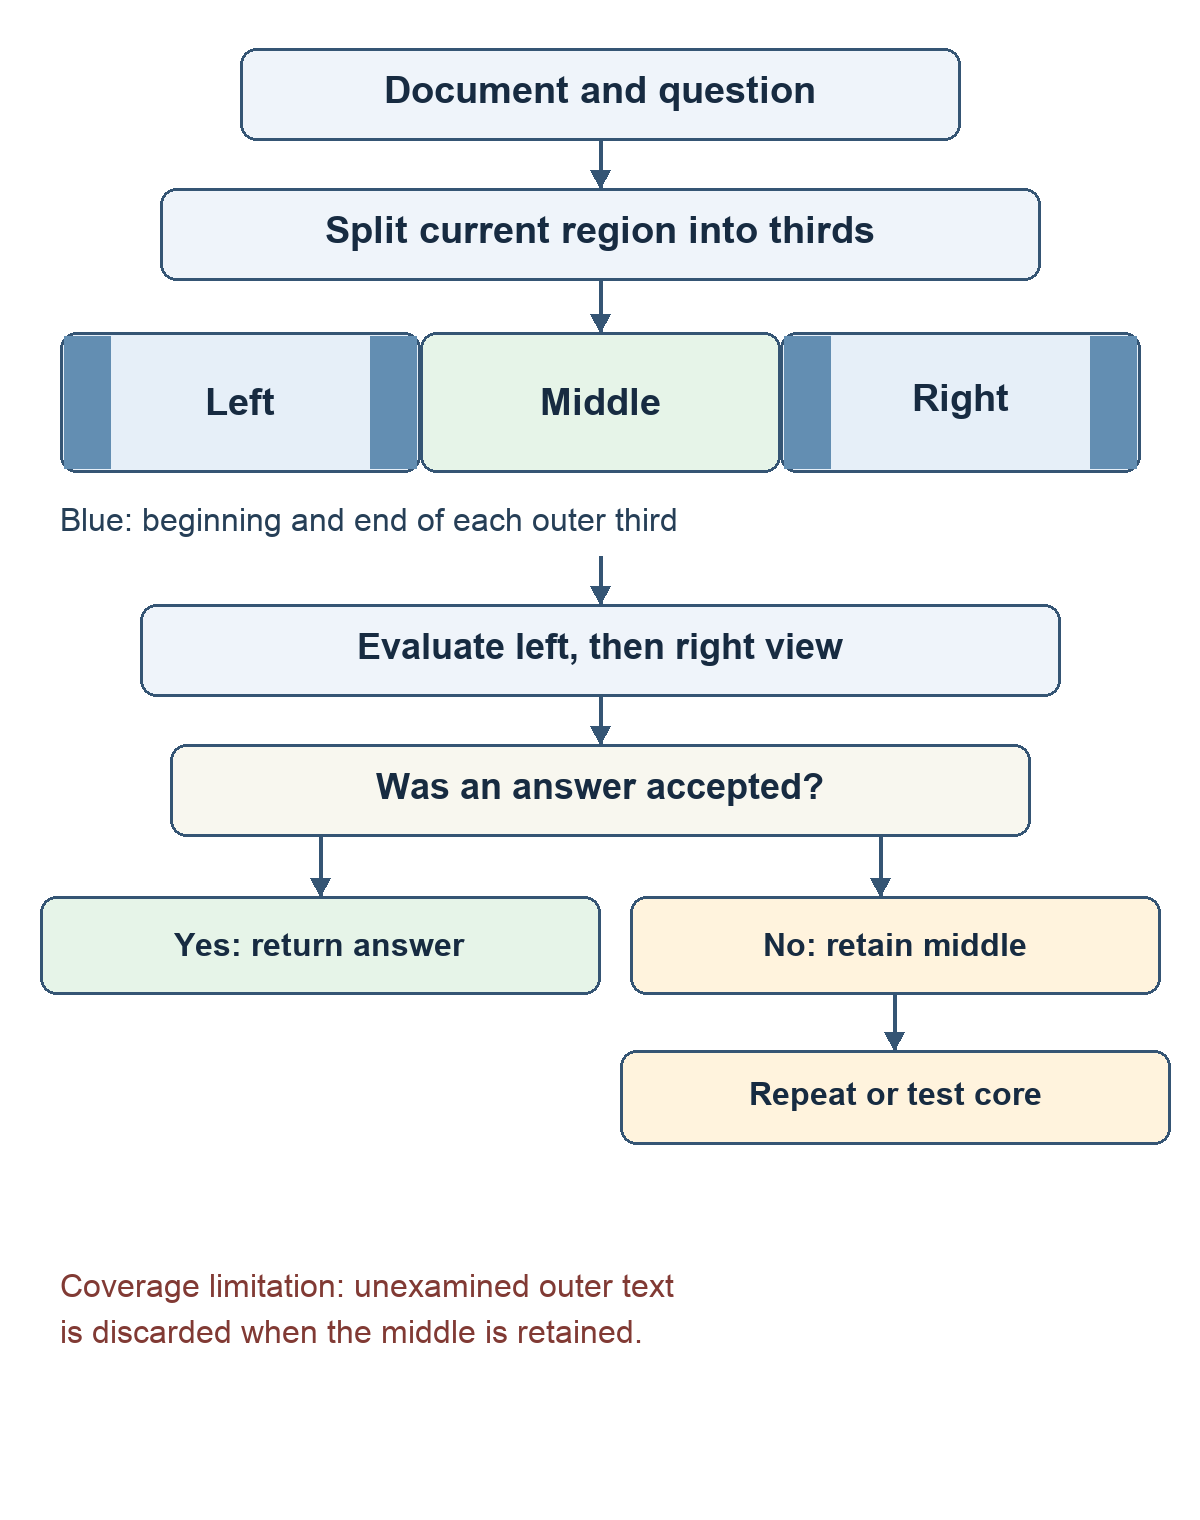
\includegraphics[width=\columnwidth]{figures.png}
\caption{Recursive boundary exposure and its coverage limitation. Outer-third views are evaluated sequentially; the middle third is retained when neither yields an accepted answer.}
\label{fig:method}
\end{figure}

Figure~\ref{fig:method} illustrates the decision process. For a shrinking region the number of recursive levels is bounded by $\min\{8,\lceil\log_3(N/500)\rceil\}$ up to integer rounding. This bounds recursion depth, not total retrieval cost or correctness: embedding, indexing, model calls, prompt processing, and generation also contribute. Evidence inside an unviewed portion of an outer third is discarded; the algorithm therefore does not guarantee that arbitrary evidence is exposed.

\subsection{Decision Rule and Failure Modes}
The procedure can be expressed through a decision function $g(q,V)$ that returns either an accepted response or the rejection symbol $\bot$. For each nonterminal region, the next state is
\begin{equation}
R_{d+1}=M_d\quad\text{if}\quad
 g(q,V(L_d))=g(q,V(R_d'))=\bot .
\end{equation}
If the first call returns an accepted response, the second call is not made. Otherwise the right view is checked, and only two rejections trigger recursion. At the terminal region the same evaluator is called once on the core. Thus, rejection is a control signal rather than evidence that all words in a third have been examined. This distinction matters whenever a third is longer than the 800-word view budget.

For example, if a 3,000-word outer region contains a relevant fact at its 1,500th word, neither the first nor last 400 words contains the fact. A negative response to that view cannot exclude the fact from the region. The subsequent choice of the middle third discards it. Even a perfect evaluator cannot recover it in that traversal. By contrast, if a model accepts an incorrect answer from an earlier view, early stopping prevents inspection of later views. Both omission and premature acceptance are therefore possible; the oracle experiment isolates only the first of these mechanisms.

An answer may require combining multiple statements. Since each boundary view is evaluated separately, a statement in the left view and another in the right view are not necessarily available together to a single call. The same problem arises if the beginning and end of a long third are concatenated without the intervening text: local references and qualifying statements can be lost. The method is consequently most directly suited to questions answerable from a single examined view, and the present evaluation does not demonstrate reliability for multi-hop synthesis.

\subsection{Comparison Systems}
The benchmark forms overlapping 256-word passages with a 48-word overlap. BM25 ranks them using $k_1=1.5$ and $b=0.75$; dense retrieval ranks by cosine similarity of query and passage embeddings. The hybrid score is $0.8$ times cosine similarity plus $0.2$ times the fraction of unique question terms found in the passage. Each baseline selects up to eight passages and restores document order before generating a single answer. This hybrid is an experimental score combination, not BM25 plus dense retrieval. Passage overlap means that measured input word counts can include repetitions.

The lexical and dense baselines make different assumptions. BM25 rewards matches between question terms and passage terms while adjusting for document frequency and passage length. Dense cosine similarity compares semantic vector representations and can, in principle, surface passages with less direct lexical overlap. The combined score retains both semantic similarity and a simple measure of question-term coverage, although the relative scales of its two components are not calibrated. Baseline results should therefore be understood as results for these particular configurations rather than definitive statements about entire families of retrieval methods.

\section{Dataset and Experimental Setup}
\subsection{LongBench Pilot}
We use the English MultiFieldQA file from LongBench \cite{bai}. Of its 150 examples, 122 have contexts of at least 2,000 whitespace-separated words. Ten were sampled with Python's random seed 42; their contexts span 2,076--7,551 words, with a median of 2,831. This subset is not the full benchmark and excludes shorter contexts. The dataset was obtained from a public LongBench mirror (SHA-256: \texttt{0aac182fd317dcf6d74f8e1e0f3e6102}\allowbreak\texttt{9407435346c2e0b3ff9fb45ae49c5c3f}). The sampling procedure and model settings are specified here to support independent replication.

The local Ollama generator was \texttt{llama3.2:latest} (recorded model ID \texttt{a80c4f17acd5}) and the embedding model was \texttt{nomic-embed-text:latest} (ID \texttt{0a109f422b47}). Generation used temperature zero. Baselines used an 8,192-token context setting and a 100-token output limit; the boundary evaluator used a 4,096-token setting and a 256-token output limit. Prompts also differed. No hardware specification is recorded, limiting reproducibility of timing results.

\subsection{Measures}
Answer token F1 is calculated after lowercasing, punctuation and English article removal, and whitespace normalization, using the best score among reference answers. For normalized predicted and reference token multisets $P$ and $G$, the F1 score is $2|P\cap G|/(|P|+|G|)$ when both are nonempty. We report mean per-question F1, total words supplied across generator calls, number of calls, and median generator-call elapsed time. Word counts are not model-token counts; call timings exclude embedding, indexing, and retrieval scoring. Fixed method order and caching confound timing comparisons. F1 is neither evidence recall nor a measure of factual faithfulness \cite{ragas,ares}.

\subsection{Evaluation Protocol}
For every sampled question, all four configurations were applied to the same context and reference answers. The comparison is paired at the question level, but the reported table consists of aggregate descriptive statistics rather than estimates of paired statistical significance. Each retrieval baseline generates once after passage selection. The boundary condition can invoke the model repeatedly, and the total number of presented words accumulates across those calls. A lower mean word count does not imply a lower total inference cost because model initialization, prompt processing, and response generation are not captured by this count alone.

The token-overlap measure rewards shared normalized words and can assign partial credit to an incomplete answer. It can also penalize an accurate paraphrase or overvalue a response that contains some correct words alongside unsupported details. Multiple reference answers, when present, are handled by retaining the best F1. A response represented by \texttt{NOT\_FOUND} is treated as an ordinary prediction for scoring. Abstention counts are reported separately to make one common failure pattern visible; they do not by themselves distinguish appropriate abstention from missed evidence.

\subsection{Synthetic Exposure Test}
A separate synthetic test relocates a single inserted secret phrase to 21 equally spaced positions from 0\% to 100\% in an approximately 21,400-word historical background document. It tests two queries: a lexical query sharing words with the inserted sentence and a paraphrase. An oracle marks a hit if the exact phrase appears in an examined view; there are no language-model calls. The comparators are the top BM25 passage, one fixed beginning/end view, and full-text exposure. This is a coverage diagnostic rather than a QA accuracy benchmark. The original background source and its distribution rights were not recorded; this limits independent replication of this diagnostic.

The synthetic design places the same sentence at controlled positions while holding the surrounding background fixed. This allows the coverage consequences of changing position to be observed without relying on the language model to recognize the answer. The lexical and paraphrase queries influence BM25 ranking, but the boundary exposure procedure itself is position based. The full-document condition necessarily exposes the inserted phrase and serves only as a coverage ceiling. All 21 placements belong to the same background and should not be interpreted as independent samples from a broad population of documents.

\section{Results}
\begin{table}[t]
\caption{LongBench pilot results ($n=10$). Words and calls are means; time is median generator-call elapsed time.}
\label{tab:pilot}\centering\footnotesize
\begin{tabular}{lrrrr}\toprule
Method & F1 (\%) & Words & Calls & Time (s)\\\midrule
BM25 & 28.67 & 2037 & 1.0 & 11.52\\
Dense & 29.75 & 2040 & 1.0 & 8.67\\
Hybrid & 26.45 & 2037 & 1.0 & 5.68\\
RBR-style & 27.21 & 1837 & 3.4 & 13.41\\\bottomrule
\end{tabular}\end{table}
\begin{figure}[t]
\centering
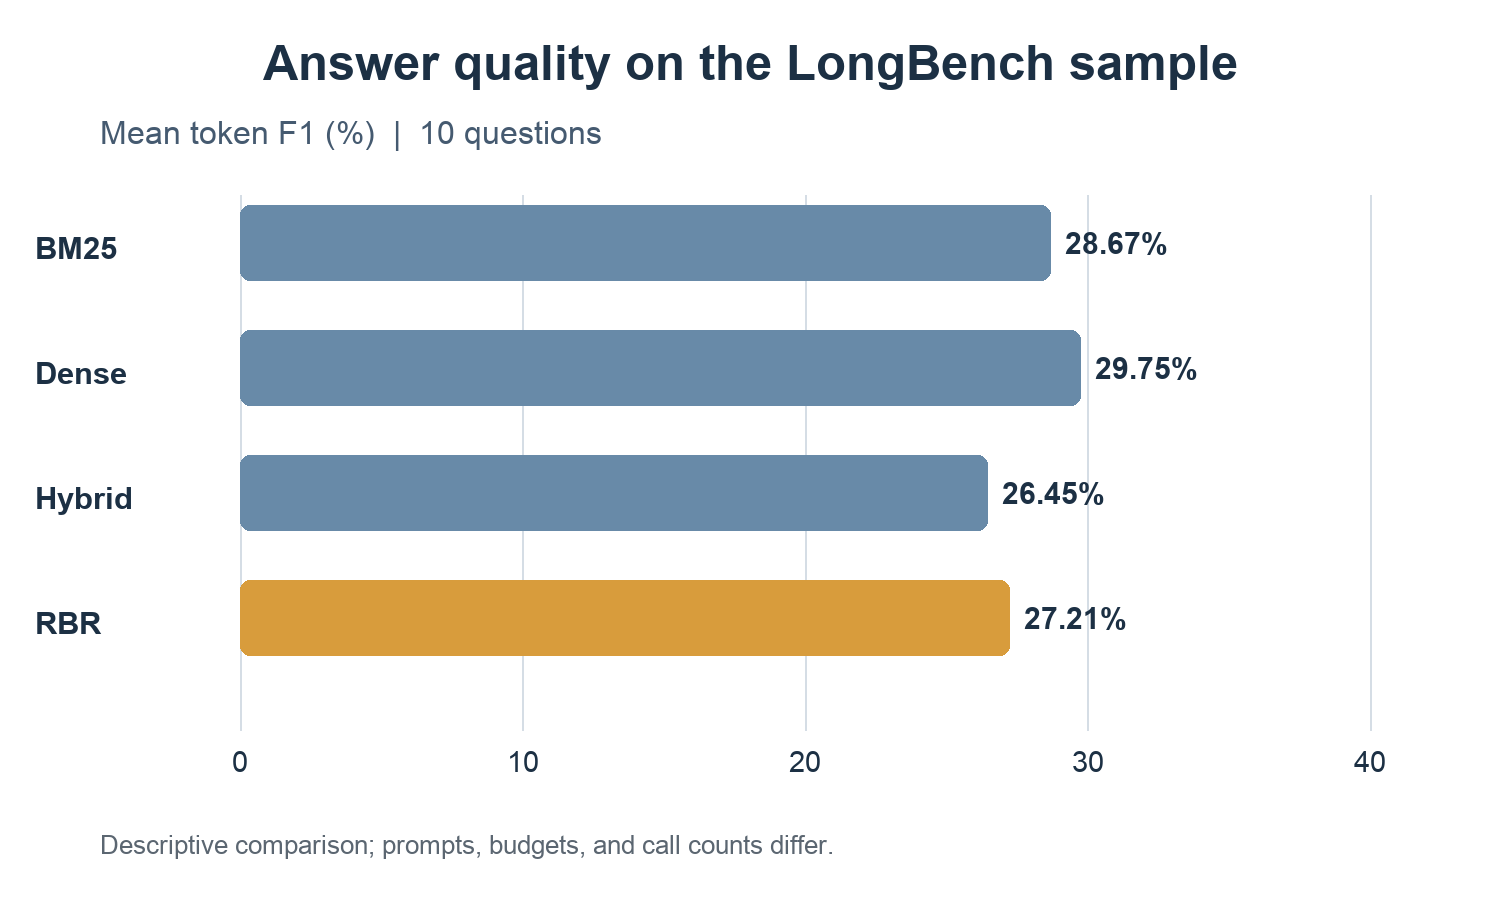
\includegraphics[width=\columnwidth]{benchmark_f1.png}
\caption{Mean answer token F1 on the ten-question LongBench sample. The configurations differ in prompts, context budgets, and model calls.}
\label{fig:f1}
\end{figure}

Table~\ref{tab:pilot} and Fig.~\ref{fig:f1} report descriptive results only. Dense retrieval had the largest observed mean F1; the differences are not evidence of a stable ranking. Boundary peeling made more calls on average and passed fewer total context words on average, but the differing prompts and context limits prevent attributing these differences to the traversal alone. The recorded numbers of \texttt{NOT\_FOUND} responses were 4, 4, 5, and 5 for BM25, dense, hybrid, and RBR-style methods, respectively. No significance test, confidence interval, or human assessment was performed.

\begin{table}[t]
\caption{Synthetic exact-phrase exposure hits out of 21 positions. Full exposure is an oracle coverage reference, not a model baseline.}
\label{tab:coverage}\centering\footnotesize
\begin{tabular}{lrr}\toprule
Exposure method & Lexical query & Paraphrase query\\\midrule
RBR oracle & 7 & 7\\
BM25 top passage & 21 & 0\\
Fixed boundary view & 2 & 2\\
Full document & 21 & 21\\\bottomrule
\end{tabular}\end{table}
\begin{figure}[t]
\centering
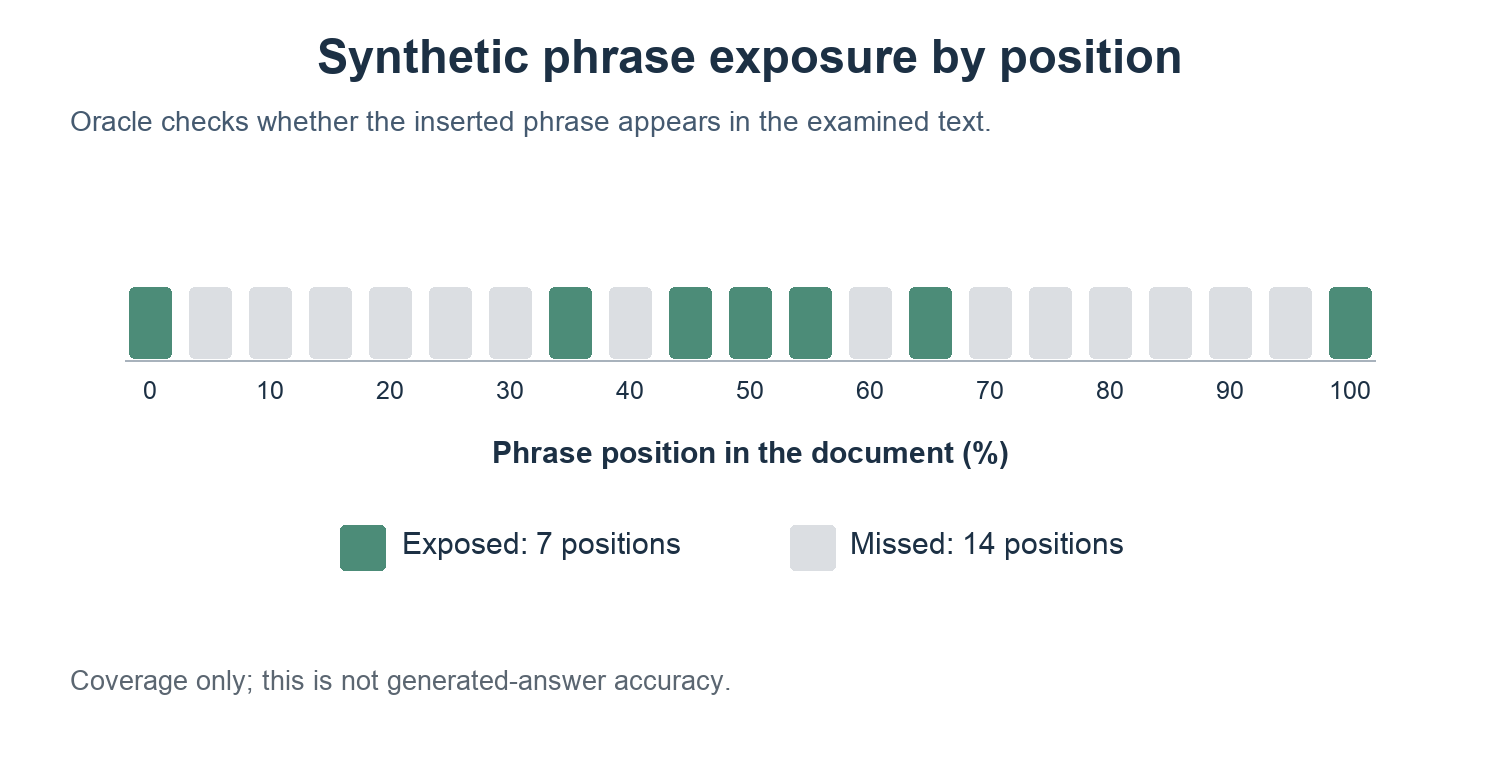
\includegraphics[width=\columnwidth]{position_coverage.png}
\caption{Oracle exposure of the inserted phrase at 21 positions in one background document. A hit indicates visibility in a boundary view, not answer correctness.}
\label{fig:positions}
\end{figure}

As Table~\ref{tab:coverage} and Fig.~\ref{fig:positions} show, the boundary strategy misses 14 of the 21 positions even with a perfect phrase-detection oracle. Both query variants have the same boundary exposure because that procedure does not use query relevance to select views. BM25's different outcomes illustrate dependence on lexical overlap for these specific queries; they should not be generalized to all paraphrases. The synthetic test does not measure a model's ability to answer, and its full-document condition does not imply successful long-context generation.

\subsection{Interpretation of Answer Quality}
The absolute difference between the largest and smallest observed mean F1 values is 3.30 percentage points, and the difference between dense retrieval and boundary peeling is 2.54 points. These descriptive differences are small relative to the uncertainty expected from ten heterogeneous questions. They are also affected by system-level differences beyond retrieval, including the evaluator instruction and output budget. The results therefore cannot establish either equivalence or superiority.

The four systems abstained frequently. This could reflect missing or insufficient context, the generator's response to its instructions, difficulties with the question, or a mismatch between a generated answer and the reference. The aggregate record does not identify the cause for every example. In particular, an answer string occurring in a selected passage is not equivalent to evidence that the passage supports the reference answer, so string presence alone should not be treated as annotated retrieval recall.

\subsection{Interpretation of Exposure}
The oracle's seven successful positions demonstrate that recursively exposing portions of the middle can extend coverage beyond a fixed beginning/end view, which exposed the phrase at two positions in this experiment. At the same time, fourteen positions remained unexposed. This comparison describes only the selected positions, one inserted sentence, and one document. It does not prove that all real evidence is equally likely to be distributed across positions, nor does it measure whether the language model would answer correctly when shown the phrase.

\section{Discussion and Limitations}
The coverage experiment exposes a structural failure mode: detecting no answer in a bounded view does not establish absence from the entire third. Early acceptance can also return an unsupported answer. These risks are amplified when evidence spans multiple passages or depends on context outside the view. An exhaustive or overlap-aware fallback, relevance-guided candidate inspection, and evidence verification are possible extensions, but were not evaluated here.

The real-data experiment uses one model, one embedding model, ten questions, unequal prompts and budgets, and sequential fixed-order execution. No full-context generation baseline or annotated evidence-recall measurement is available. Model service versions and hardware were not recorded fully. Results should not be compared directly to official LongBench leaderboard scores. Further evaluation should use more examples and seeds, multiple models, matched prompts and budgets, randomized execution order, a full-context baseline where feasible, and human or independently validated evidence and faithfulness assessments \cite{beir,ares}. Timing should include indexing and retrieval and disclose hardware.

\subsection{Directions for a Controlled Study}
A stronger follow-up should predefine a test set and report both overall performance and results by context length, answer location, and question type. A paired bootstrap interval over examples, together with paired comparisons between methods, would better describe uncertainty than raw means alone. Repeated generations and multiple model configurations would help identify sensitivity to model choice and inference variation. Such analysis should specify any intended statistical claims before inspecting the results.

To isolate the effect of context selection, future comparisons should use the same generator, answer instructions, output limits, and total context budget where feasible. A full-context condition should be included for contexts that fit the model, with any truncation or exclusion stated explicitly. Because recursive evaluation uses multiple calls, studies should report both equal-input-budget and equal-call-budget comparisons rather than assuming that either captures all deployment costs. Model warm-up, caching, hardware, and execution order should be controlled or disclosed.

Coverage-aware variants could inspect all subwindows of an outer third before discarding it, retain high-relevance passages for a final answer, or combine position-based and retrieval-ranked views. Such alternatives introduce additional calls or indexing cost and may change the error profile. They are research proposals rather than results of the present experiment. Evidence annotations and human review would be needed to determine whether an answer is actually supported, especially when questions require combining facts from different regions.

\section{Conclusion}
Recursive boundary exposure offers a simple way to present progressively central regions to a language model. In the available LongBench pilot it achieved 27.21\% mean token F1; the small and uncontrolled comparison cannot establish whether it outperforms other approaches. The separate oracle experiment shows that the current bounded-view design can discard unexamined evidence, motivating coverage-aware revisions and a larger controlled evaluation.

\begin{thebibliography}{99}
\bibitem{liu} N. F. Liu \emph{et al.}, ``Lost in the middle: How language models use long contexts,'' \emph{Trans. Assoc. Comput. Linguistics}, vol. 12, pp. 157--173, 2024, doi: 10.1162/tacl\_a\_00638.
\bibitem{lewis} P. Lewis \emph{et al.}, ``Retrieval-augmented generation for knowledge-intensive NLP tasks,'' in \emph{Adv. Neural Inf. Process. Syst.}, vol. 33, 2020, pp. 9459--9474.
\bibitem{robertson} S. Robertson and H. Zaragoza, ``The probabilistic relevance framework: BM25 and beyond,'' \emph{Found. Trends Inf. Retr.}, vol. 3, no. 4, pp. 333--389, 2009, doi: 10.1561/1500000019.
\bibitem{karpukhin} V. Karpukhin \emph{et al.}, ``Dense passage retrieval for open-domain question answering,'' in \emph{Proc. EMNLP}, 2020, pp. 6769--6781, doi: 10.18653/v1/2020.emnlp-main.550.
\bibitem{reimers} N. Reimers and I. Gurevych, ``Sentence-BERT: Sentence embeddings using Siamese BERT-networks,'' in \emph{Proc. EMNLP-IJCNLP}, 2019, pp. 3982--3992, doi: 10.18653/v1/D19-1410.
\bibitem{beir} N. Thakur \emph{et al.}, ``BEIR: A heterogeneous benchmark for zero-shot evaluation of information retrieval models,'' in \emph{Proc. NeurIPS Datasets and Benchmarks Track}, 2021. [Online]. Available: \url{https://arxiv.org/abs/2104.08663}
\bibitem{bai} Y. Bai \emph{et al.}, ``LongBench: A bilingual, multitask benchmark for long context understanding,'' in \emph{Proc. ACL}, 2024, pp. 3119--3137, doi: 10.18653/v1/2024.acl-long.172.
\bibitem{li} Z. Li \emph{et al.}, ``Retrieval augmented generation or long-context LLMs? A comprehensive study and hybrid approach,'' in \emph{Proc. EMNLP: Industry Track}, 2024, pp. 881--893. [Online]. Available: \url{https://aclanthology.org/2024.emnlp-industry.66/}
\bibitem{kwiatkowski} T. Kwiatkowski \emph{et al.}, ``Natural questions: A benchmark for question answering research,'' \emph{Trans. Assoc. Comput. Linguistics}, vol. 7, pp. 453--466, 2019, doi: 10.1162/tacl\_a\_00276.
\bibitem{ragas} S. Es \emph{et al.}, ``RAGAs: Automated evaluation of retrieval augmented generation,'' in \emph{Proc. EACL: System Demonstrations}, 2024. [Online]. Available: \url{https://aclanthology.org/2024.eacl-demo.16/}
\bibitem{ares} J. Saad-Falcon \emph{et al.}, ``ARES: An automated evaluation framework for retrieval-augmented generation systems,'' in \emph{Proc. NAACL}, 2024. [Online]. Available: \url{https://aclanthology.org/2024.naacl-long.20/}
\bibitem{chen} Y. Chen \emph{et al.}, ``LongLoRA: Efficient fine-tuning of long-context large language models,'' 2023. [Online]. Available: \url{https://arxiv.org/abs/2309.12307}
\end{thebibliography}
\end{document}
